\documentclass[a4paper]{article} 
\usepackage{graphicx} 
\usepackage[ngerman]{babel} 
\usepackage[ansinew]{inputenc} 
\usepackage[T1]{fontenc} 
\usepackage{tgpagella} 
\usepackage{geometry} 
\usepackage{color} 
\usepackage{microtype} 
\usepackage{minted}
\usepackage{caption}
\usepackage[headsepline,footsepline]{scrpage2}
\usepackage{textcomp}
\usepackage{pdfpages}
\usepackage{mdframed}



\makeatletter
\renewcommand\minted@pygmentize[2][\jobname.pyg]{
  \def\minted@cmd{pygmentize -l #2 -f latex -F tokenmerge
    \minted@opt{gobble} \minted@opt{texcl} \minted@opt{mathescape}
    \minted@opt{startinline} \minted@opt{funcnamehighlighting}
    \minted@opt{linenos} -P "verboptions=\minted@opt{extra}"
    -O encoding=UTF-8,outencoding=iso-8859-1 -o \jobname.out.pyg #1}
  \immediate\write18{\minted@cmd}
  % For debugging, uncomment:
  %\immediate\typeout{\minted@cmd}
  \ifthenelse{\equal{\minted@opt@bgcolor}{}}
   {}
   {\begin{minted@colorbg}{\minted@opt@bgcolor}}
  \input{\jobname.out.pyg}
  \ifthenelse{\equal{\minted@opt@bgcolor}{}}
   {}
   {\end{minted@colorbg}}
  \DeleteFile{\jobname.out.pyg}}
\makeatother


\title{Dokumentation - 6 Übung}
\author{Roman Lumetsberger}
\date{\today}

\newmintedfile[ccode]{cpp}{
               linenos,
               numbersep=5pt,
               frame=lines,
               framesep=2mm
}

\newmintedfile[javacode]{java}{
               linenos,
               numbersep=5pt,
               frame=lines,
               tabsize=2,
               framesep=2mm,
}
\newmintedfile[csscode]{css}{
               linenos,
               numbersep=5pt,
               frame=lines,
               tabsize=2,
               framesep=2mm,
}
\newmintedfile[sqlcode]{sql}{
               linenos,
               numbersep=5pt,
               frame=lines,
               tabsize=2,
               framesep=2mm,
}
\captionsetup{
  font=footnotesize,
  justification=raggedright,
  singlelinecheck=false
}


\newcommand{\srcDir}{../Beispiel/src/at/lumetsnet/caas/}
\newcommand{\testDir}{../Beispiel/test/at/lumetsnet/caas/test/}

\definecolor{lineColor}{RGB}{151,0,0}
\pagestyle{scrheadings}
\clearscrheadfoot
\begin{document}
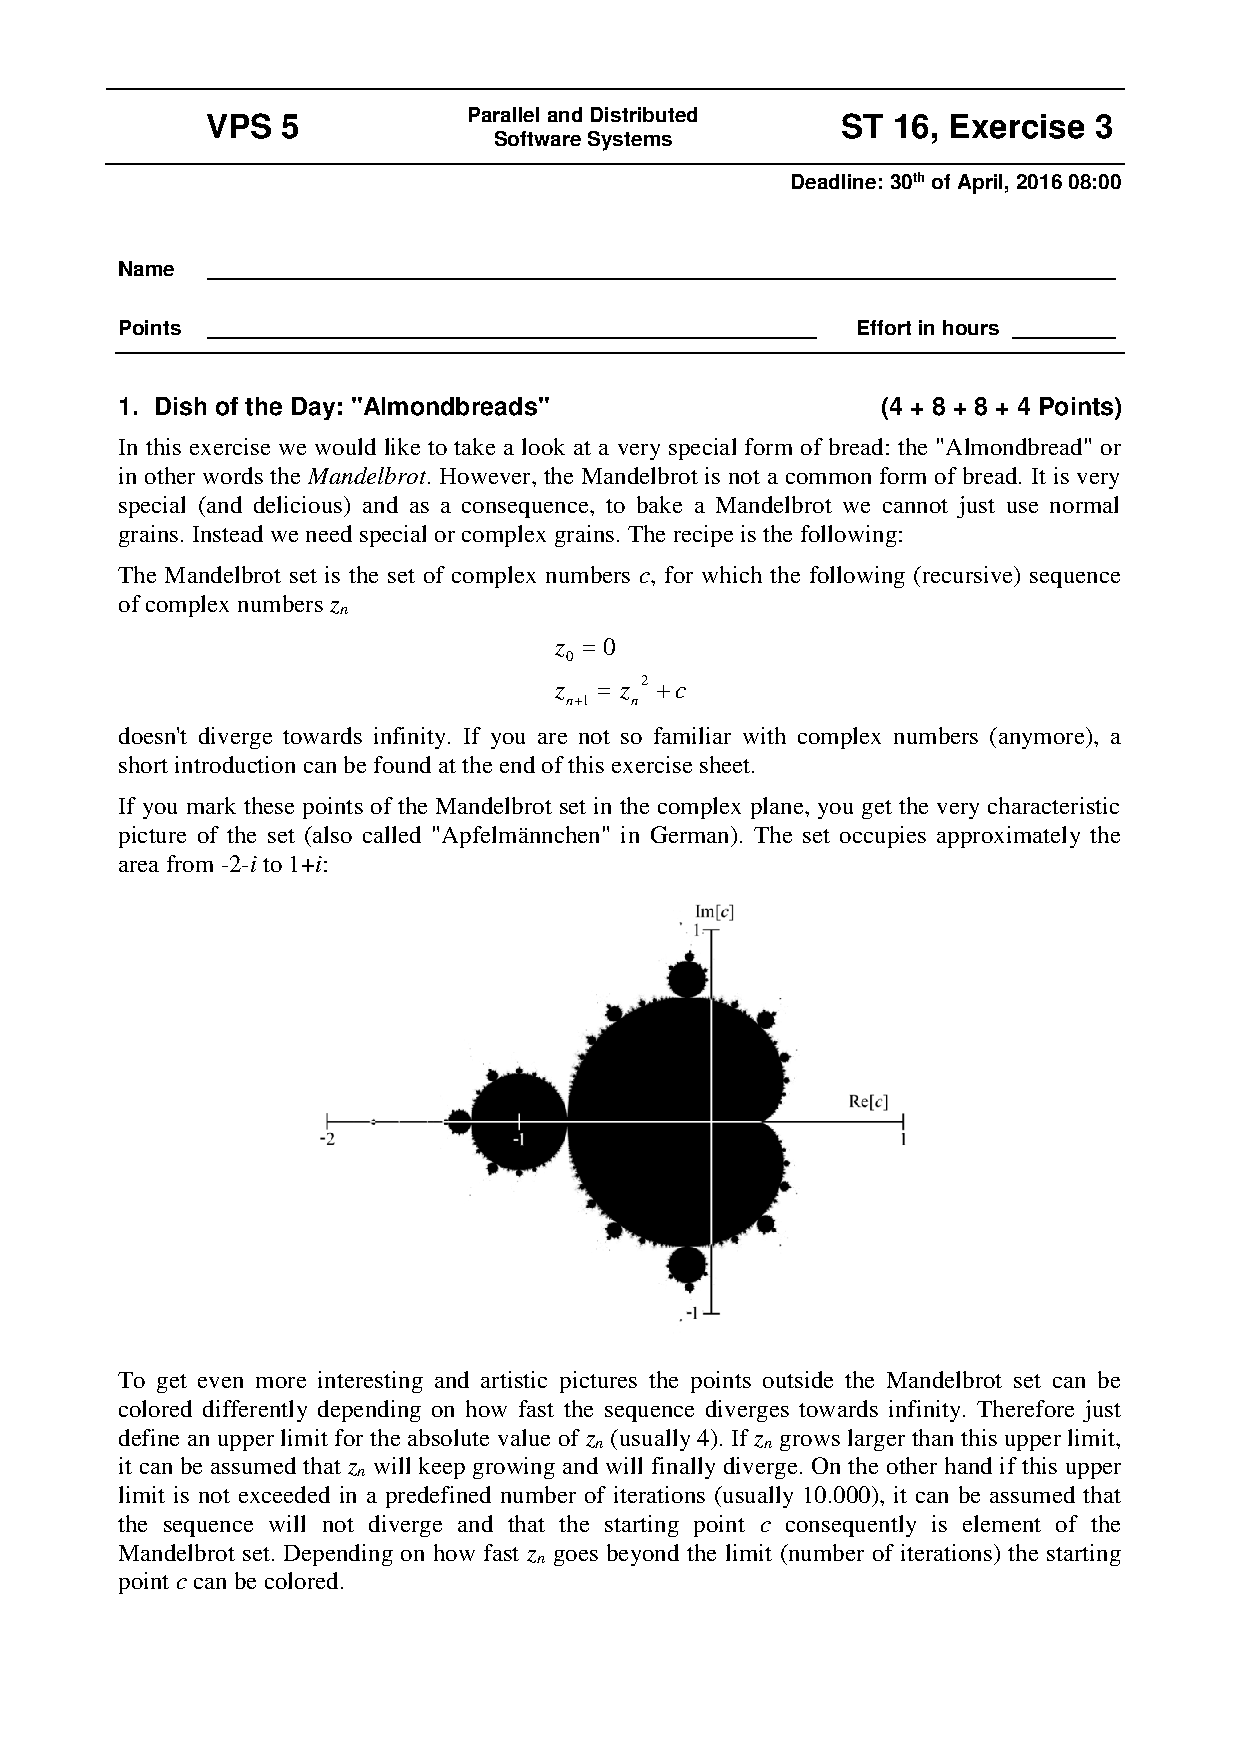
\includepdf[pages=-]{angabe.pdf}

\ihead{VPS SS 2016 - �bung 03}
\ifoot{Roman Lumetsberger}
\cfoot{1310307026}
\ofoot{Seite \pagemark}

\section{Dish of the Day: ""Almondbreads""}
\subsection*{1a. Generator}
Der Generator wurde bereits in der �bung programmiert und baut auf vorhandenem Code auf.

\cscode{\srcDir/MandelbrotGenerator/SyncImageGenerator.cs}

\subsection*{1b. Asynchrone Implementierung}
Um asynchrone Implementierungen zu erm�glichen, wurde das Interface \texttt{IImageGenerator} um das Event \texttt{ImageGenerated} erweitert. Weiters muss bei der Zuweisung des Ergebnisses an die GUI der Thread gewechselt werden.

Die folgenden Implementierungen leiten vom originalen \texttt{SyncImageGenerator} ab und verlagern die Arbeit in den Hintergrund. Dabei wurde eine einfache M�glichkeit zum Abbrechen der Berechnung implementiert. Hierzu wurde die Implementierung um ein simples Stop-Flag erweitert. (Code siehe 1.a)

\subsubsection*{Implementierung 1: \texttt{AsyncImageGenerator}}
Bei dieser Implementierung wurden \texttt{Threads} verwendet, um die Arbeit in den Hintergrund zu verlagern. Die Pr�fung ob bereits eine Berechnung l�uft, wird �ber die Abfrage des Thread-Status \texttt{IsAlive} durchgef�hrt. Ist noch eine Berechnung aktiv, wird das Stop-Flag gesetzt und dann auf die Beendigung des Threads gewartet.
\emph{Anmerkung: } Auf die Beendigung wird am GUI-Thread gewartet, da der Hintergrundthread bei jedem Schleifendurchgang pr�ft, ob das Stop-Flag gesetzt ist. Diese Zeitspanne ist sehr kurz und verursacht somit kein Einfrieren der Oberfl�che.

\cscode{\srcDir/MandelbrotGenerator/AsyncImageGenerator.cs}

\subsubsection*{Implementierung 2: \texttt{AsyncWorkerImageGenerator}}
Die \texttt{AsyncWorkerImageGenerator} Implementierung verwendet einen .NET \texttt{BackgroundWorker}, um die Arbeit in den Hintergrund zu verlagern. Die Ergebnisweiergabe wird �ber das Event \texttt{RunWorkerCompleted} und die Eigenschaft \texttt{Result} abgewickelt. Die Synchronisierung der Berechnungen wird �ber die Eigenschaft \texttt{IsBusy} der Klasse \texttt{BackgroundWorker} gel�st.

\cscode{\srcDir/MandelbrotGenerator/AsyncWorkerImageGenerator.cs}

\subsection*{1c. Parallele Version}
Die Aufteilung der Arbeit auf die Worker kann zeilenweise erfolgen. Dabei wird die ben�tigte Anzahl an Worker-Threads erzeugt, wobei jeder dieser Threads immer eine Zeile berechnet. Sobald alle Zeilen berechnet sind, werden die Threads beendet. Diese Aufteilung hat den Vorteil, dass die Threads ungef�hr gleich ausgelastet sind, da zwei benachbarte Zeilen ungef�hr den selben Rechnaufwand verursachen.

Zur Verwaltung der Berechnung wird ein zus�tzlicher Management-Thread verwendet. Dieser �bernimmt die Zeitmessung und das Aul�sen des Events. 
Der Zugriff auf das Bitmap wird mit Hilfe von Locks gesichert. 

\cscode{\srcDir/MandelbrotGenerator/ParallelImageGenerator.cs}

\subsection*{1d. Performance}
\subsubsection*{Parameter}
\begin{itemize}
\item Ausschnitt: -1,4-0,1i bis -1,32-0,02i
\item Aufl�sung: 800x600
\item WorkerThreads: 8 (parallele Implementierung)
\end{itemize}

\begin{table}[!htb]
\centering
\caption{Ergebnisse}
\begin{tabular}{ccc}
\hline
\multicolumn{3}{c}{Simulation} \\ \cline{1-3}                                                                                 
Lauf & Sync [ms] & Parallel [ms] \\ \cline{1-3}
1 & 2832 & 603 \\
2 & 2817 & 595 \\
3 & 2829 & 617 \\
4 & 2822 & 583 \\
5 & 2819 & 592 \\
6 & 2828 & 612 \\
7 & 2834 & 600 \\
8 & 2822 & 619 \\
9 & 2823 & 606 \\
10 & 2844 & 599 \\ \cline{1-3}
\textbf{�}    & \textbf{2827} & \textbf{599} \\
Std. Abw.    & 7,73      & 10,73

\end{tabular}
\end{table} 

\begin{itemize}
\item SpeedUp: 4,69
\end{itemize}


\end{document}